\documentclass[11pt]{article}

\usepackage[a4paper,margin=1in]{geometry}
\usepackage{amsmath,amssymb,amsfonts,amsthm}
\usepackage{bm}
\usepackage{graphicx}
\usepackage{siunitx}
\usepackage{mathtools}
\usepackage{tikz}
\usepackage{hyperref}
\usepackage{enumitem}
\usepackage{booktabs}
\usepackage{caption}
\usepackage{subcaption}
\usepackage{physics}
\usepackage{microtype}
\usepackage{cleveref}

\title{Numerical Methods for the Heat Equation on Non-Uniform, Non-Quadrilateral Grids: A Finite Volume Approach}
\author{}
\date{}

\theoremstyle{plain}
\newtheorem{theorem}{Theorem}[section]
\newtheorem{proposition}[theorem]{Proposition}
\newtheorem{lemma}[theorem]{Lemma}

\theoremstyle{definition}
\newtheorem{definition}[theorem]{Definition}
\newtheorem{assumption}[theorem]{Assumption}

\theoremstyle{remark}
\newtheorem{remark}[theorem]{Remark}
\numberwithin{equation}{section}

\begin{document}
\maketitle

\begin{abstract}
We present a finite volume discretization of the two-dimensional heat equation on non-uniform meshes that are not restricted to structured quadrilateral grids. The method is designed for conforming triangular and polygonal meshes and is written in a form that matches a practical sparse-matrix implementation. The spatial discretization uses control volumes built from the primal mesh geometry, with diffusive fluxes approximated by edge-based transmissibilities. On polygonal meshes an optional non-orthogonal correction augments the basic two-point flux approximation by a reconstructed-gradient term. Time integration is performed with the implicit Euler method, leading at each time step to a sparse linear system with a diagonal mass matrix and a geometry-dependent diffusion operator. Particular attention is given to the construction of the matrix entries, the role of mesh geometry in the coefficients, and the algorithmic structure of the assembly and solve stages. The resulting formulation is suitable for verification against analytical solutions and for comparison across structured square meshes, hexagonal polygonal meshes, mixed polygon meshes, and unstructured Delaunay meshes.
\end{abstract}

\section{Introduction}
The heat equation
\begin{equation}
\label{eq:heat_eq}
\partial_t u - \alpha \Delta u = 0
\qquad \text{in } \Omega \times (0,T]
\end{equation}
models diffusion of temperature in a homogeneous isotropic medium, where $u=u(\bm{x},t)$ is temperature, $\alpha>0$ is thermal diffusivity, and $\Omega \subset \mathbb{R}^2$ is the spatial domain.

On a uniform Cartesian mesh, the spatial operator is usually represented by the standard five-point stencil. That approach is simple because all cells have the same area, the same face lengths, and the same distances to neighbouring unknowns. On non-uniform or non-quadrilateral meshes, none of these quantities are constant. A practical method must therefore compute the local geometric weights directly from the mesh.

The finite volume method is a natural choice in this setting because it preserves local conservation: the rate of change of heat in a control volume equals the sum of fluxes through its boundary. The present document formalizes the discrete scheme used in the accompanying solver implementation, with emphasis on:
\begin{enumerate}[label=\arabic*.]
\item the geometric construction of control volumes,
\item the derivation of the matrix entries from flux balances,
\item the sparse assembly algorithm,
\item the implicit time-stepping procedure, and
\item the interpretation of the method on general meshes.
\end{enumerate}

\section{Model Problem}
Let $\Omega$ be a bounded Lipschitz domain with boundary $\partial \Omega = \Gamma_D \cup \Gamma_N$, where $\Gamma_D \cap \Gamma_N = \varnothing$. We consider
\begin{align}
\partial_t u - \alpha \Delta u &= 0 && \text{in } \Omega \times (0,T], \label{eq:strong_form} \\
u &= g_D && \text{on } \Gamma_D \times (0,T], \label{eq:dirichlet_bc} \\
\alpha \nabla u \cdot \bm{n} &= g_N && \text{on } \Gamma_N \times (0,T], \label{eq:neumann_bc} \\
u(\bm{x},0) &= u_0(\bm{x}) && \text{in } \Omega. \label{eq:initial_cond}
\end{align}
Here $\bm{n}$ denotes the outward unit normal on the boundary.

\subsection{Finite Volume Balance}
For a control volume $\mathcal{C}_i \subset \Omega$, integrating \cref{eq:strong_form} over $\mathcal{C}_i$ and applying the divergence theorem gives
\begin{equation}
\label{eq:fvm_balance}
\frac{d}{dt} \int_{\mathcal{C}_i} u \, dA
- \alpha \int_{\partial \mathcal{C}_i} \nabla u \cdot \bm{n} \, ds = 0.
\end{equation}
This is the starting point of the scheme. The discrete method replaces the volume integral by a control-volume mass term and replaces the boundary integral by a sum of numerical fluxes over the interfaces of $\mathcal{C}_i$.

\section{Mesh and Control Volumes}
\subsection{Primal Mesh}
Two mesh families are considered in the implementation.
\begin{enumerate}[label=\arabic*.]
\item A vertex-centred scheme on an unstructured triangular mesh $\mathcal{T}_h$.
\item A cell-centred scheme on a conforming polygonal mesh, including square, hexagonal, and mixed polygon meshes.
\end{enumerate}

In both cases the method is edge-based: neighbouring unknowns interact only if their control volumes share an interface of positive length.

\subsection{Vertex-Centred Triangular Control Volumes}
Let $\mathcal{T}_h$ be a conforming triangulation of $\Omega$ with vertices $\{\bm{x}_i\}_{i=1}^{N_v}$. Around each primal vertex $\bm{x}_i$, a median-dual control volume $\mathcal{C}_i$ is constructed by connecting triangle centroids to the midpoints of incident edges. The area of $\mathcal{C}_i$ is denoted by $A_i$.

For a triangle $K = \operatorname{conv}\{\bm{x}_i,\bm{x}_j,\bm{x}_k\}$, the centroid-based dual assigns one third of $|K|$ to each of its three vertices. Therefore
\begin{equation}
\label{eq:cv_area}
A_i = \sum_{K \ni i} \frac{|K|}{3}.
\end{equation}
This diagonal quantity becomes the local mass associated with degree of freedom $i$.

\subsection{Cell-Centred Polygonal Control Volumes}
For a conforming polygonal mesh $\{\mathcal{P}_i\}_{i=1}^{N_c}$, each polygon is already a control volume. The unknown is associated with the polygon centroid and the control-volume area is simply
\begin{equation}
|\mathcal{P}_i| = \text{area of polygon } \mathcal{P}_i.
\end{equation}
The polygonal extension follows the same balance law as the triangular case, but the indexing is by cells rather than primal vertices.

\section{Edge Flux Approximation}
\subsection{Neighbour Relations}
Let $\mathcal{N}(i)$ denote the set of neighbours of degree of freedom $i$. In the triangular vertex-centred scheme, $j \in \mathcal{N}(i)$ if vertices $i$ and $j$ share a primal edge. In the polygonal cell-centred scheme, $j \in \mathcal{N}(i)$ if polygons $\mathcal{P}_i$ and $\mathcal{P}_j$ share a full edge.

For each neighbouring pair $(i,j)$, we define:
\begin{itemize}
\item an interface length $|\gamma_{ij}|$,
\item a centre-to-centre distance $d_{ij}$,
\item a transmissibility coefficient
\begin{equation}
\label{eq:transmissibility}
T_{ij} = \frac{|\gamma_{ij}|}{d_{ij}}.
\end{equation}
\end{itemize}

\subsection{Triangular Median-Dual Geometry}
For the triangular scheme, the interface between neighbouring control volumes is a dual segment associated with the primal edge $E_{ij}$. In the implementation, $|\gamma_{ij}|$ is computed from the local triangle geometry by summing, for each adjacent triangle, the perpendicular distance from the triangle centroid to the midpoint of $E_{ij}$. Thus
\begin{equation}
\label{eq:dual_length}
|\gamma_{ij}| \approx \sum_{K \supset E_{ij}} 2 \, \left| (\bm{c}_K - \bm{m}_{ij}) \cdot \bm{n}_{ij} \right|,
\end{equation}
where $\bm{c}_K$ is the centroid of triangle $K$, $\bm{m}_{ij}$ is the midpoint of the primal edge, and $\bm{n}_{ij}$ is a unit normal to that edge.

\subsection{Polygonal Interface Geometry}
For the polygonal scheme, $|\gamma_{ij}|$ is simply the length of the shared polygon edge, and $d_{ij}$ is the Euclidean distance between the centroids of the two neighbouring cells.

\subsection{Two-Point Flux Approximation}
The diffusive flux from control volume $i$ to control volume $j$ is approximated by
\begin{equation}
\label{eq:tpfa_flux}
F_{ij} = - \alpha T_{ij}(u_j - u_i).
\end{equation}
This is the standard two-point flux approximation (TPFA). It is exact on orthogonal meshes for linear solutions and remains a consistent first-order approximation on sufficiently regular non-orthogonal meshes.

Summing the fluxes over all interfaces of $\mathcal{C}_i$ gives the discrete diffusion contribution
\begin{equation}
\label{eq:discrete_flux_sum}
-\alpha \int_{\partial \mathcal{C}_i} \nabla u \cdot \bm{n} \, ds
\approx \sum_{j \in \mathcal{N}(i)} F_{ij}
= -\alpha \sum_{j \in \mathcal{N}(i)} T_{ij}(u_j - u_i).
\end{equation}

\subsection{Non-Orthogonal Correction on Polygonal Meshes}
The polygonal solver optionally augments the TPFA flux when the line joining neighbouring cell centroids is not aligned with the face normal. Let two polygonal cells $\mathcal{P}_i$ and $\mathcal{P}_j$ share an edge $e_{ij}$ of length $|e_{ij}|$. Let $\bm{c}_i$ and $\bm{c}_j$ be the cell centroids and let $\bm{n}_{ij}$ be the unit normal on $e_{ij}$ oriented from cell $i$ toward cell $j$ so that
\begin{equation}
\label{eq:dn_def}
d_{n,ij} = (\bm{c}_j - \bm{c}_i) \cdot \bm{n}_{ij} > 0.
\end{equation}
The exact flux through the common face is
\begin{equation}
\label{eq:exact_face_flux}
F_{ij} = - \alpha |e_{ij}| \, \nabla u(\bm{x}_{ij}) \cdot \bm{n}_{ij},
\end{equation}
where $\bm{x}_{ij}$ is any representative point on the face, for example the face midpoint.

The key observation is that the face normal can be decomposed into a component aligned with the centroid connector and a residual component:
\begin{equation}
\label{eq:normal_decomposition}
\bm{n}_{ij}
= \frac{\bm{c}_j - \bm{c}_i}{d_{n,ij}}
  + \left(
      \bm{n}_{ij}
      - \frac{\bm{c}_j - \bm{c}_i}{d_{n,ij}}
    \right).
\end{equation}
Substituting \cref{eq:normal_decomposition} into \cref{eq:exact_face_flux} yields the split
\begin{equation}
\label{eq:flux_split}
F_{ij} = F_{ij}^{\mathrm{orth}} + F_{ij}^{\mathrm{corr}},
\end{equation}
with
\begin{align}
F_{ij}^{\mathrm{orth}}
&= - \alpha |e_{ij}| \,
\nabla u(\bm{x}_{ij}) \cdot
\frac{\bm{c}_j - \bm{c}_i}{d_{n,ij}},
\label{eq:orth_flux_exact} \\
F_{ij}^{\mathrm{corr}}
&= - \alpha |e_{ij}| \,
\nabla u(\bm{x}_{ij}) \cdot
\left(
\bm{n}_{ij} - \frac{\bm{c}_j - \bm{c}_i}{d_{n,ij}}
\right).
\label{eq:corr_flux_exact}
\end{align}

The first term is approximated by a two-point difference:
\begin{equation}
\label{eq:orth_flux_discrete}
F_{ij}^{\mathrm{orth}}
\approx
- \alpha |e_{ij}| \frac{u_j - u_i}{d_{n,ij}}.
\end{equation}
This is exactly the coefficient used by the code when the correction is disabled. On an orthogonal mesh, $\bm{c}_j - \bm{c}_i$ is parallel to $\bm{n}_{ij}$, so the residual vector in \cref{eq:corr_flux_exact} vanishes and the scheme reduces to pure TPFA.

To approximate the correction term, the implementation reconstructs a cellwise gradient by weighted least squares. For a cell $i$ with neighbours $\mathcal{N}(i)$, define the offset vectors
\begin{equation}
\bm{r}_{ik} = \bm{c}_k - \bm{c}_i,
\qquad k \in \mathcal{N}(i),
\end{equation}
and let
\begin{equation}
w_{ik} = \frac{1}{\norm{\bm{r}_{ik}}^2}.
\end{equation}
The reconstructed gradient $\bm{g}_i \approx \nabla u(\bm{c}_i)$ is the minimizer of
\begin{equation}
\label{eq:wls_problem}
\bm{g}_i
= \operatorname*{arg\,min}_{\bm{g} \in \mathbb{R}^2}
\sum_{k \in \mathcal{N}(i)}
w_{ik}
\left(
u_k - u_i - \bm{g} \cdot \bm{r}_{ik}
\right)^2.
\end{equation}
The associated normal equations are
\begin{equation}
\label{eq:wls_normal_equations}
G_i \bm{g}_i
=
\sum_{k \in \mathcal{N}(i)}
w_{ik} (u_k - u_i)\bm{r}_{ik},
\qquad
G_i =
\sum_{k \in \mathcal{N}(i)}
w_{ik}\,\bm{r}_{ik}\bm{r}_{ik}^{\top}.
\end{equation}
Whenever $G_i$ is nonsingular, the reconstruction can be written as a linear combination of neighbouring unknowns:
\begin{equation}
\label{eq:gradient_linear_form}
\bm{g}_i
=
\sum_{m \in \{i\} \cup \mathcal{N}(i)}
\bm{\beta}_{im} u_m,
\end{equation}
where the coefficient vectors $\bm{\beta}_{im} \in \mathbb{R}^2$ are precomputed once during assembly. This is the role of the gradient-reconstruction operator in the code.

The face gradient is then approximated by the arithmetic average
\begin{equation}
\label{eq:face_gradient_average}
\widehat{\nabla u}_{ij}
= \frac{1}{2}(\bm{g}_i + \bm{g}_j),
\end{equation}
and the correction term becomes
\begin{equation}
\label{eq:corr_flux_discrete}
F_{ij}^{\mathrm{corr}}
\approx
- \alpha |e_{ij}|
\widehat{\nabla u}_{ij} \cdot
\left(
\bm{n}_{ij} - \frac{\bm{c}_j - \bm{c}_i}{d_{n,ij}}
\right).
\end{equation}
Combining \cref{eq:orth_flux_discrete,eq:corr_flux_discrete}, the discrete face flux used by the polygonal solver is
\begin{equation}
\label{eq:full_corrected_flux}
F_{ij}
\approx
- \alpha |e_{ij}| \frac{u_j - u_i}{d_{n,ij}}
- \alpha |e_{ij}|
\widehat{\nabla u}_{ij} \cdot
\left(
\bm{n}_{ij} - \frac{\bm{c}_j - \bm{c}_i}{d_{n,ij}}
\right).
\end{equation}
The first term is the orthogonal TPFA part. The second term corrects the flux when the mesh is skew or non-orthogonal.

\begin{figure}[t]
\centering
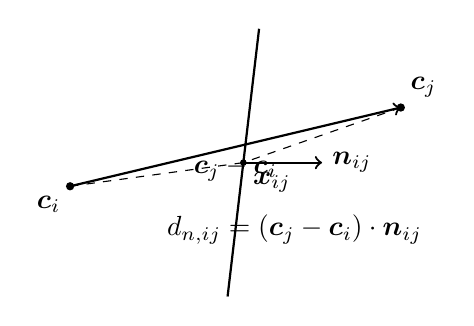
\begin{tikzpicture}[scale=1.0]
\coordinate (ci) at (0,0);
\coordinate (cj) at (4.2,1.0);
\coordinate (m) at (2.2,0.3);
\coordinate (a) at (2.0,-1.4);
\coordinate (b) at (2.4,2.0);
\draw[thick] (a) -- (b);
\fill (ci) circle (1.5pt) node[below left] {$\bm{c}_i$};
\fill (cj) circle (1.5pt) node[above right] {$\bm{c}_j$};
\fill (m) circle (1.2pt) node[below right] {$\bm{x}_{ij}$};
\draw[->,thick] (ci) -- (cj) node[midway,below] {$\bm{c}_j-\bm{c}_i$};
\draw[->,thick] (m) -- ++(1.0,0.0) node[right] {$\bm{n}_{ij}$};
\draw[dashed] (ci) -- (m);
\draw[dashed] (cj) -- (m);
\node at (2.85,-0.55) {$d_{n,ij}=(\bm{c}_j-\bm{c}_i)\cdot \bm{n}_{ij}$};
\end{tikzpicture}
\caption{Geometry of one polygonal interface. On an orthogonal mesh the centroid connector is parallel to the face normal; otherwise the residual direction in \cref{eq:normal_decomposition} is nonzero and a correction term is added.}
\label{fig:nonorth_geometry}
\end{figure}

\section{Semi-Discrete Matrix Form}
\subsection{Local Balance Equation}
Approximating the mean value of $u$ over $\mathcal{C}_i$ by the discrete unknown $u_i(t)$, the finite volume balance becomes
\begin{equation}
\label{eq:semi_discrete_balance}
A_i \frac{d u_i}{dt}
- \alpha \sum_{j \in \mathcal{N}(i)} T_{ij}(u_j - u_i)
= b_i(t),
\end{equation}
where $A_i$ is the control-volume area and $b_i(t)$ contains boundary contributions.
For the polygonal solver with the correction enabled, the interface contribution is more generally interpreted as a sum of corrected face fluxes $F_{ij}$ from \cref{eq:full_corrected_flux}; \cref{eq:semi_discrete_balance} then represents the same balance law written in compact operator form.

\subsection{Mass Matrix}
The mass matrix is diagonal because each control volume contributes only to its own degree of freedom:
\begin{equation}
\label{eq:mass_matrix}
M_{ij} =
\begin{cases}
A_i, & i=j, \\
0, & i \neq j.
\end{cases}
\end{equation}
In code, this is stored as a sparse diagonal matrix.

\subsection{Diffusion Matrix}
The diffusion matrix is assembled edge by edge. For every neighbouring pair $(i,j)$, the orthogonal TPFA part contributes the off-diagonal coupling
\begin{equation}
\label{eq:offdiag_entry}
A_{ij} = - \alpha T_{ij}, \qquad i \neq j,
\end{equation}
and the diagonal entry is the sum of outgoing transmissibilities:
\begin{equation}
\label{eq:diag_entry}
A_{ii} = \alpha \sum_{j \in \mathcal{N}(i)} T_{ij}.
\end{equation}
Thus the assembled matrix satisfies
\begin{equation}
\label{eq:row_sum_form}
(A \bm{u})_i = \alpha \sum_{j \in \mathcal{N}(i)} T_{ij}(u_i - u_j).
\end{equation}
For pure TPFA this operator is symmetric. In the polygonal solver with the optional non-orthogonal correction enabled, the global operator is split as
\begin{equation}
\label{eq:operator_split}
A = A^{\mathrm{orth}} + A^{\mathrm{corr}},
\end{equation}
where $A^{\mathrm{orth}}$ is assembled from the standard $2 \times 2$ TPFA blocks and $A^{\mathrm{corr}}$ contains the gradient-reconstruction terms induced by \cref{eq:full_corrected_flux}. The correction enlarges the stencil beyond the immediate pair $(i,j)$ because $\bm{g}_i$ and $\bm{g}_j$ depend on neighbouring cell values through \cref{eq:gradient_linear_form}. Consequently, the corrected polygonal operator is conservative but need not remain symmetric.

More explicitly, let
\begin{equation}
\label{eq:correction_direction}
\bm{q}_{ij}
=
\bm{n}_{ij} - \frac{\bm{c}_j - \bm{c}_i}{d_{n,ij}}.
\end{equation}
If the cellwise reconstructions are written as $\bm{g}_i = \sum_m \bm{\beta}_{im} u_m$ and $\bm{g}_j = \sum_m \bm{\beta}_{jm} u_m$, then the averaged face gradient gives
\begin{equation}
\widehat{\nabla u}_{ij} \cdot \bm{q}_{ij}
=
\sum_m \eta_{ijm} u_m,
\qquad
\eta_{ijm}
=
\frac{1}{2}\left(
\bm{q}_{ij} \cdot \bm{\beta}_{im}
+ \bm{q}_{ij} \cdot \bm{\beta}_{jm}
\right).
\end{equation}
Therefore the correction flux can be written as
\begin{equation}
\label{eq:correction_flux_matrix_form}
F_{ij}^{\mathrm{corr}}
=
- \alpha |e_{ij}| \sum_m \eta_{ijm} u_m.
\end{equation}
In matrix assembly, this flux is inserted conservatively by subtracting \cref{eq:correction_flux_matrix_form} from row $i$ and adding it to row $j$. This is exactly the algebraic pattern used in the implementation.

\subsection{How the Matrix is Created in Practice}
The matrix construction is most easily understood by looking at a single edge contribution. For an interior neighbour pair $(i,j)$:
\begin{enumerate}[label=\arabic*.]
\item Compute the interface length $|\gamma_{ij}|$.
\item Compute the oriented face normal $\bm{n}_{ij}$ and the projected normal distance $d_{n,ij} = (\bm{c}_j-\bm{c}_i)\cdot\bm{n}_{ij}$.
\item Form the orthogonal coefficient $T_{ij}^{\mathrm{orth}} = |\gamma_{ij}|/d_{n,ij}$.
\item Add the $2 \times 2$ local block
\begin{equation}
\label{eq:local_block}
\alpha T_{ij}^{\mathrm{orth}}
\begin{bmatrix}
1 & -1 \\
-1 & 1
\end{bmatrix}
\end{equation}
to the global matrix rows and columns corresponding to $i$ and $j$.
\item If the non-orthogonal correction is enabled, reconstruct $\bm{g}_i$ and $\bm{g}_j$ from \cref{eq:wls_normal_equations}, average them as in \cref{eq:face_gradient_average}, and distribute the correction term \cref{eq:correction_flux_matrix_form} to all unknowns appearing in the local reconstructions.
\end{enumerate}

For the orthogonal TPFA part, each interface adds the same coefficient to both diagonal entries and the negative of that coefficient to the matching off-diagonal entries. Summing these edge contributions over the mesh yields a sparse symmetric matrix whose nonzero pattern follows the neighbour graph of the mesh. The optional correction adds extra couplings to neighbouring cells through the reconstruction coefficients $\bm{\beta}_{im}$ and $\bm{\beta}_{jm}$, so the corrected polygonal matrix has a wider stencil and is generally only mildly nonsymmetric.

\subsection{Resulting Semi-Discrete System}
Collecting all unknowns into $\bm{u}(t)$ gives
\begin{equation}
\label{eq:semi_discrete_matrix}
M \frac{d\bm{u}}{dt} + A \bm{u} = \bm{b}(t).
\end{equation}
This is the natural finite volume analogue of the standard semi-discrete heat equation on a structured grid, with the key difference that both $M$ and $A$ now depend on local mesh geometry.

\section{Time Discretization}
\subsection{Implicit Euler}
Let $t^n = n \Delta t$ and let $\bm{u}^n$ approximate $\bm{u}(t^n)$. Applying implicit Euler to \cref{eq:semi_discrete_matrix} gives
\begin{equation}
\label{eq:implicit_euler}
M \frac{\bm{u}^{n+1} - \bm{u}^n}{\Delta t} + A \bm{u}^{n+1} = \bm{b}^{n+1}.
\end{equation}
Rearranging,
\begin{equation}
\label{eq:linear_system}
\left( \frac{1}{\Delta t} M + A \right) \bm{u}^{n+1}
= \frac{1}{\Delta t} M \bm{u}^n + \bm{b}^{n+1}.
\end{equation}
Each time step therefore requires the solution of one sparse linear system.

\subsection{Boundary Conditions in Matrix Form}
For Dirichlet boundary conditions, the implementation replaces each boundary row of the system by an identity equation. That is, for boundary index $i$,
\begin{equation}
\label{eq:dirichlet_row}
u_i^{n+1} = g_D(\bm{x}_i, t^{n+1}).
\end{equation}
Algorithmically this means:
\begin{enumerate}[label=\arabic*.]
\item set row $i$ of the left-hand side matrix to zero,
\item set the diagonal entry $(i,i)$ to $1$,
\item set the right-hand side entry to the prescribed boundary value.
\end{enumerate}

This is exactly the modification performed in the code for both the triangular and polygonal solvers.

\section{Algorithmic Structure of the Scheme}
\subsection{Assembly Stage}
The assembly stage is time-independent for constant $\alpha$ and a fixed mesh.

\paragraph{Triangular vertex-centred solver.}
\begin{enumerate}[label=\arabic*.]
\item Read primal vertices and triangle connectivity.
\item Build the edge list and the neighbour graph.
\item Mark boundary vertices from edges with only one adjacent triangle.
\item Compute triangle centroids and triangle areas.
\item Accumulate control-volume areas $A_i$ using \cref{eq:cv_area}.
\item For each primal edge, compute the dual interface length $|\gamma_{ij}|$.
\item Form transmissibilities $T_{ij}$ and assemble the diffusion matrix edge by edge using \cref{eq:local_block}.
\item Assemble the diagonal mass matrix $M$.
\end{enumerate}

\paragraph{Polygonal cell-centred solver.}
\begin{enumerate}[label=\arabic*.]
\item Read polygon vertices and polygon connectivity.
\item Compute polygon areas and polygon centroids.
\item Detect neighbouring cells by shared polygon edges.
\item If non-orthogonal correction is enabled, precompute the weighted least-squares gradient coefficients $\bm{\beta}_{im}$ for each cell.
\item For each shared edge, compute its length, the face normal, and the projected centroid distance $d_{n,ij}$.
\item Assemble the TPFA block \cref{eq:local_block} for each interior interface.
\item If enabled, add the gradient-based correction contributions from \cref{eq:corr_flux_discrete}.
\item Form the diagonal mass matrix from polygon areas.
\end{enumerate}

\subsection{Time-Stepping Stage}
Once the matrices are assembled, the time-marching procedure is:
\begin{enumerate}[label=\arabic*.]
\item initialize $\bm{u}^0$ from the prescribed initial condition,
\item for $n=0,1,\dots,N_t-1$:
  \begin{enumerate}[label=\alph*.]
  \item build the right-hand side $(1/\Delta t) M \bm{u}^n$,
  \item insert boundary values at time $t^{n+1}$,
  \item solve the sparse linear system \cref{eq:linear_system},
  \item update $\bm{u}^{n+1}$,
  \item continue to the next step.
  \end{enumerate}
\end{enumerate}

In implementation terms, the method separates naturally into:
\begin{itemize}
\item a geometry phase,
\item a matrix assembly phase,
\item a repeated sparse solve phase.
\end{itemize}

\section{Interpretation Relative to Uniform Quadrilateral Schemes}
For readers familiar with the standard structured-grid discretization, the present method can be viewed as the same conservation law expressed with mesh-dependent coefficients.

On a uniform square mesh:
\begin{itemize}
\item all control-volume areas are equal,
\item all interior faces have the same length,
\item all neighbour distances are equal,
\item the diffusion matrix reduces to the familiar repeated stencil.
\end{itemize}

On a non-uniform mesh:
\begin{itemize}
\item the control-volume areas vary from one unknown to another,
\item the interface lengths vary,
\item the neighbour distances vary,
\item the resulting matrix entries are no longer constant.
\end{itemize}

The method is therefore not fundamentally different in principle; it is the same finite volume balance law, but with coefficients computed from local geometry rather than inherited from a uniform stencil.

\section{Stability and Qualitative Properties}
The mass matrix $M$ is diagonal with positive entries. For the purely orthogonal TPFA operator, the diffusion matrix has nonpositive off-diagonal entries, nonnegative diagonal entries, and a symmetric positive semidefinite structure. Under standard mesh regularity assumptions, this gives:
\begin{enumerate}[label=\arabic*.]
\item conservation in the interior,
\item a monotone edge-coupling structure,
\item a symmetric positive semidefinite diffusion operator,
\item a symmetric positive definite linear system after Dirichlet conditions are imposed.
\end{enumerate}
When the polygonal non-orthogonal correction is enabled, the method still preserves local conservation because each face flux enters the two adjacent balance equations with opposite signs. However, the reconstructed-gradient part can destroy symmetry and may weaken monotonicity on highly skew meshes. In that case the method should be viewed as a conservative corrected TPFA scheme rather than a strict $M$-matrix discretization. Sparse direct solvers remain appropriate, and Krylov methods for nonsymmetric systems may also be used.

\section{Analytical Verification}
The implementation is verified against analytical solutions such as:
\begin{enumerate}[label=\arabic*.]
\item the two-dimensional heat kernel,
\item a decaying sine mode,
\item a harmonic polynomial steady state.
\end{enumerate}

Given a numerical solution $u_h$ and exact solution $u$, the discrete error measures are
\begin{align}
\norm{e}_{L^2(\Omega)} &\approx \left( \sum_i A_i \, |u_h(\bm{x}_i,t) - u(\bm{x}_i,t)|^2 \right)^{1/2}, \label{eq:l2_error} \\
\norm{e}_{L^\infty(\Omega)} &\approx \max_i |u_h(\bm{x}_i,t) - u(\bm{x}_i,t)|. \label{eq:linf_error}
\end{align}
For polygonal cell-centred tests, the index $i$ runs over cells and $A_i$ denotes polygon area; for triangular vertex-centred tests, $i$ runs over dual control volumes.

\section{Conclusion}
The finite volume scheme presented here generalizes the familiar heat-equation discretization from uniform quadrilateral meshes to non-uniform triangular and polygonal meshes. The central ingredients are:
\begin{enumerate}[label=\arabic*.]
\item a control-volume area for each unknown,
\item an interface-based transmissibility for each neighbour pair,
\item a diagonal mass matrix,
\item a sparse diffusion operator assembled edge by edge, with an optional non-orthogonal correction on polygonal meshes,
\item implicit Euler time stepping.
\end{enumerate}

This formulation is both mathematically transparent and implementation-ready. It is therefore suitable for internal publication, code review, and further extensions such as higher-order reconstructions and anisotropic diffusion.

\section*{Acknowledgments}
The formulation follows standard finite volume principles for diffusion problems on general meshes and benefits from the classical literature on conservative discretizations of elliptic and parabolic equations.

\begin{thebibliography}{9}
\bibitem{leveque}
R. J. LeVeque, \emph{Finite Volume Methods for Hyperbolic Problems}, Cambridge University Press, 2002.

\bibitem{eymard}
R. Eymard, T. Gallou\"et, R. Herbin, \emph{Finite Volume Methods}, in: Handbook of Numerical Analysis, Vol. VII, North-Holland, 2000.

\bibitem{quarteroni}
A. Quarteroni, R. Sacco, F. Saleri, \emph{Numerical Mathematics}, Springer, 2007.

\bibitem{evans}
L. C. Evans, \emph{Partial Differential Equations}, AMS, 2010.
\end{thebibliography}

\end{document}
